\chapter{Assembling}
\section{Hardware assembling}
\paragraph{} Responsible team members: Devarsh Sheladiya, Shibichakaravarthy Senthil

\paragraph{} The rover came in a kit form. As mentioned earlier, it consists of motors, servos, wheels, and body details. Figures \ref{fig:Assembl1}, \ref{fig:Assembl2} and \ref{fig:Assembl3} demonstrate some of the assembling stages.


\begin{figure}[ht]
    \vspace{0.4cm}
    \centering
    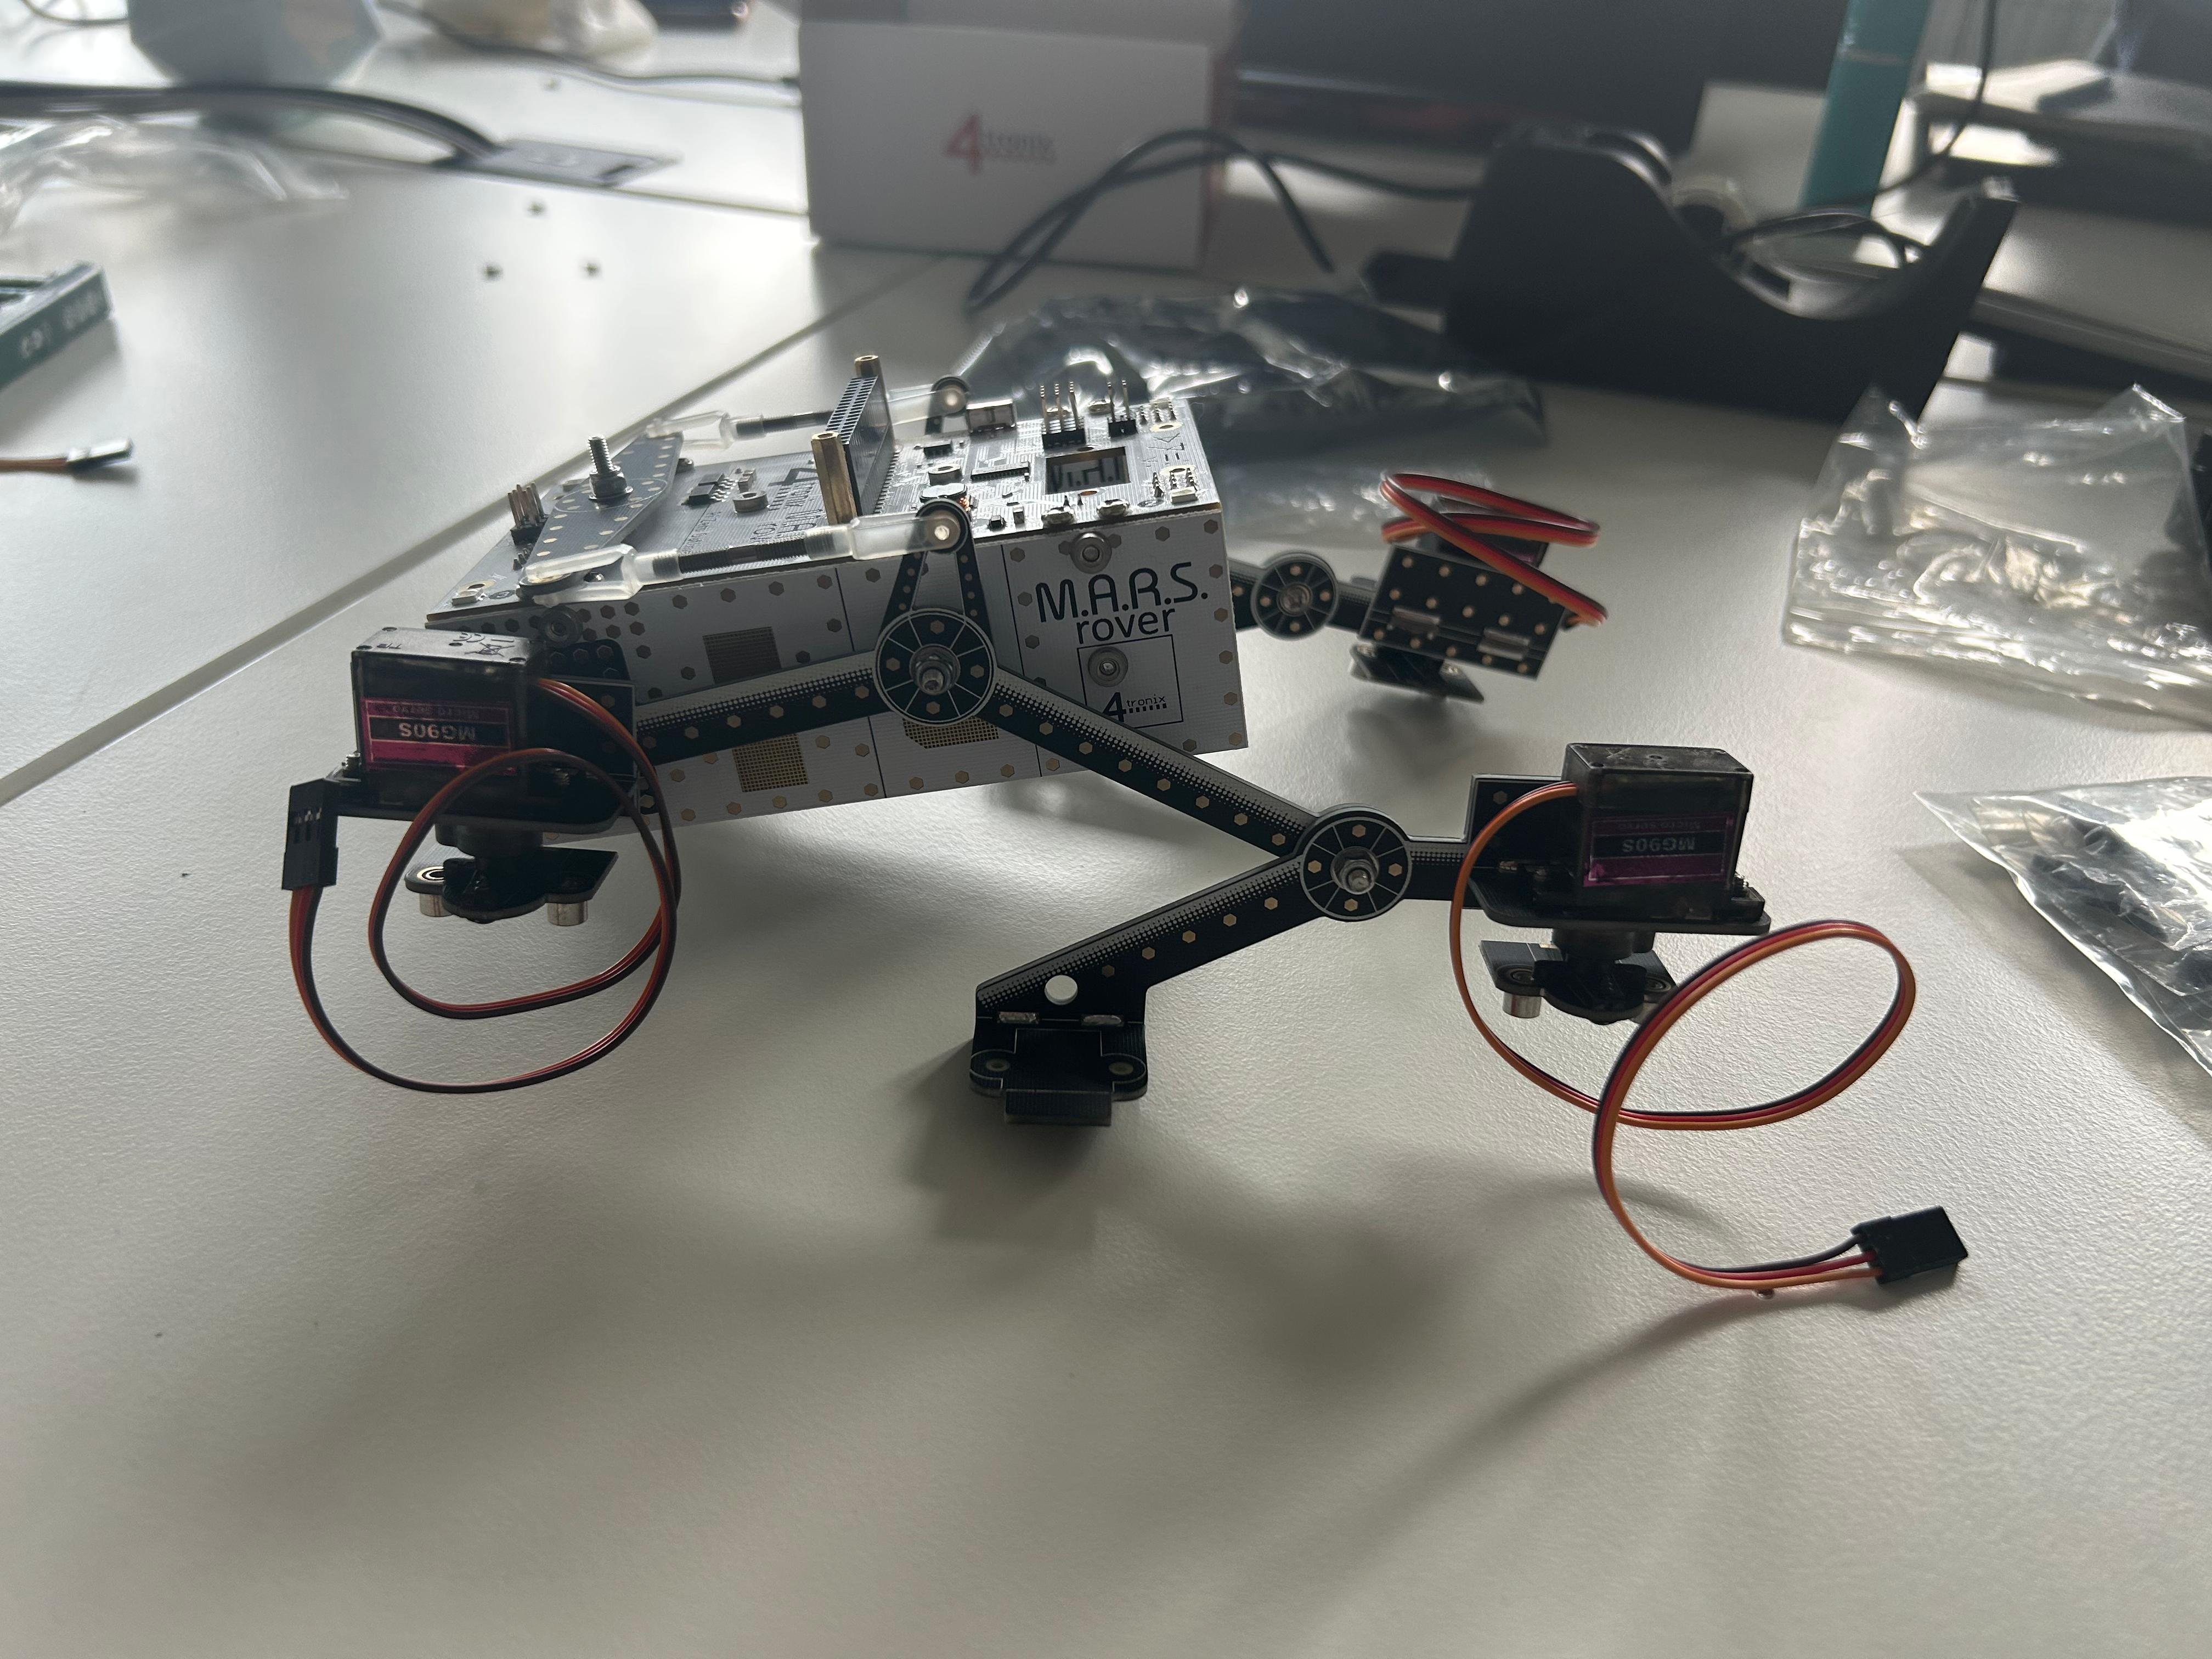
\includegraphics[width=0.48\textwidth]{Hauptkapitel/Pictures/As1.jpg}
    \caption{}
    \label{fig:Assembl1}
\end{figure}

\begin{minipage}{0.46\textwidth}
    \vspace{0.4cm}
    \centering
    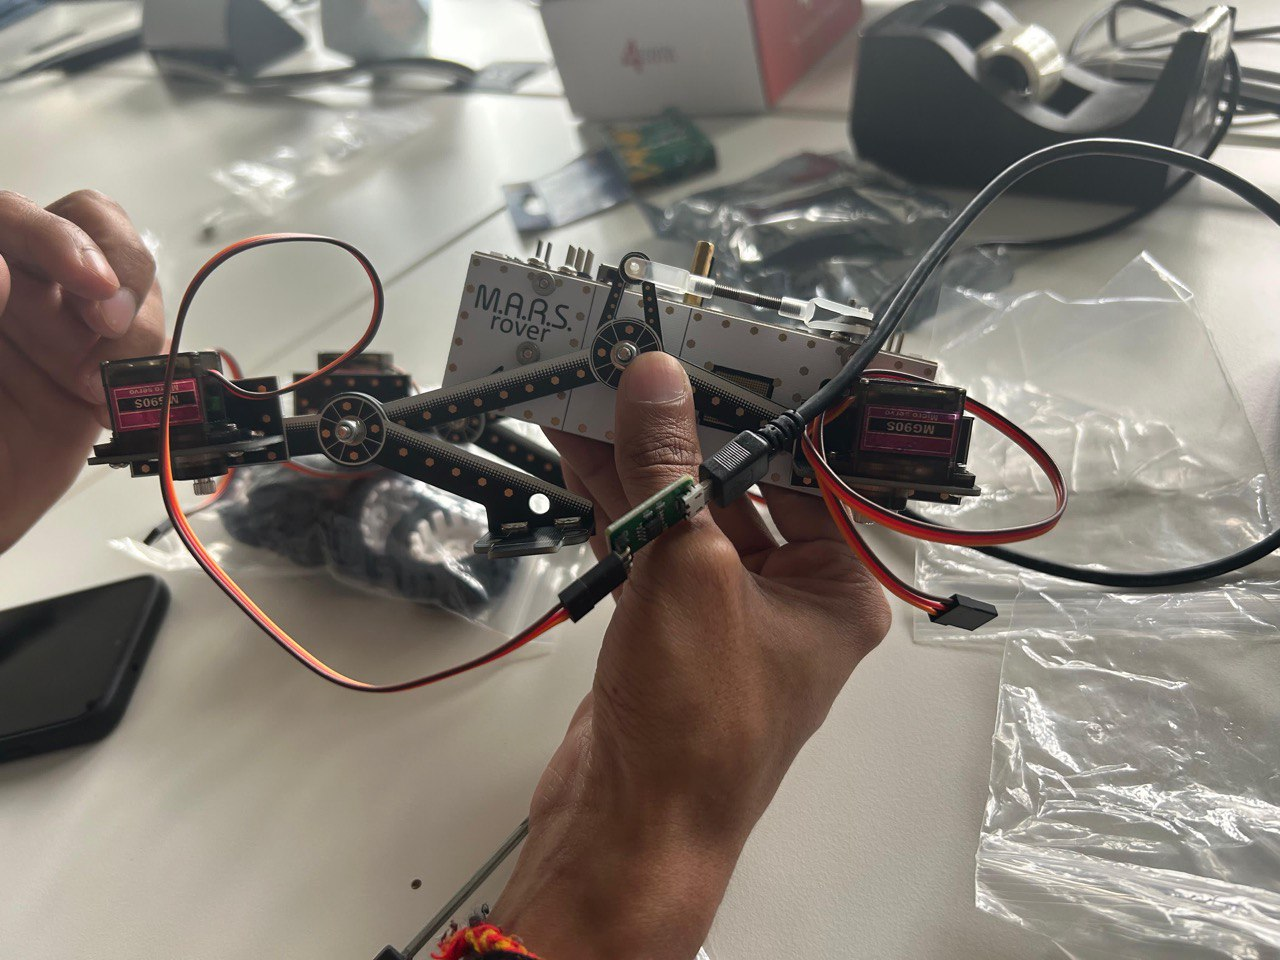
\includegraphics[width=\textwidth]{Hauptkapitel/Pictures/As2.jpg}
    \captionof{figure}{}
    \label{fig:Assembl2}
\end{minipage}
\hfill
\begin{minipage}{0.46\textwidth}
    \vspace{0.4cm}
    \centering
    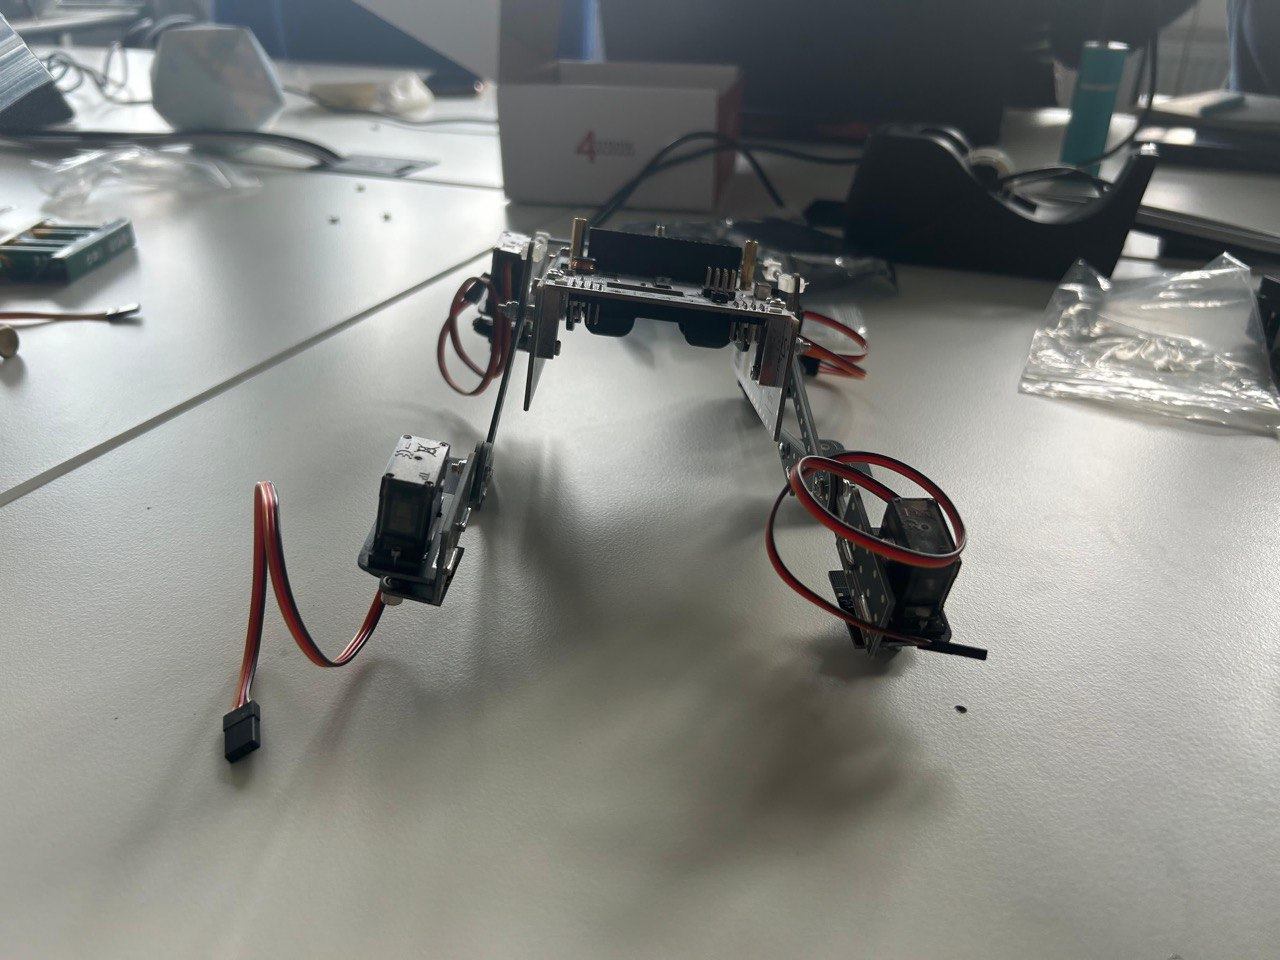
\includegraphics[width=\textwidth]{Hauptkapitel/Pictures/As3.jpg}
    \captionof{figure}{}
    \label{fig:Assembl3}
\end{minipage}

\paragraph{}Once the hardware assembly was completed, preliminary tests were conducted to verify that all components were functioning correctly. This included checking motor movement and sensor readings.

\section{Camera installation}

\paragraph{}The original Curiosity Rover has 17 cameras on board, which was the biggest number used in such a project \cite{nasa:camera}. The rover uses them to take pictures of the Mars environment.  
\paragraph{} To increase the project's potential it was decided to install a camera on the rover. The mast has a special place where the camera can be installed and it is perfectly adjusted for Raspberry Pi Camera Module 3 that was provided for our project. The figure \ref{fig:cam_rover} below demonstrates installed camera. 
 \begin{figure}[h]
     \vspace{0.4cm}
     \centering
     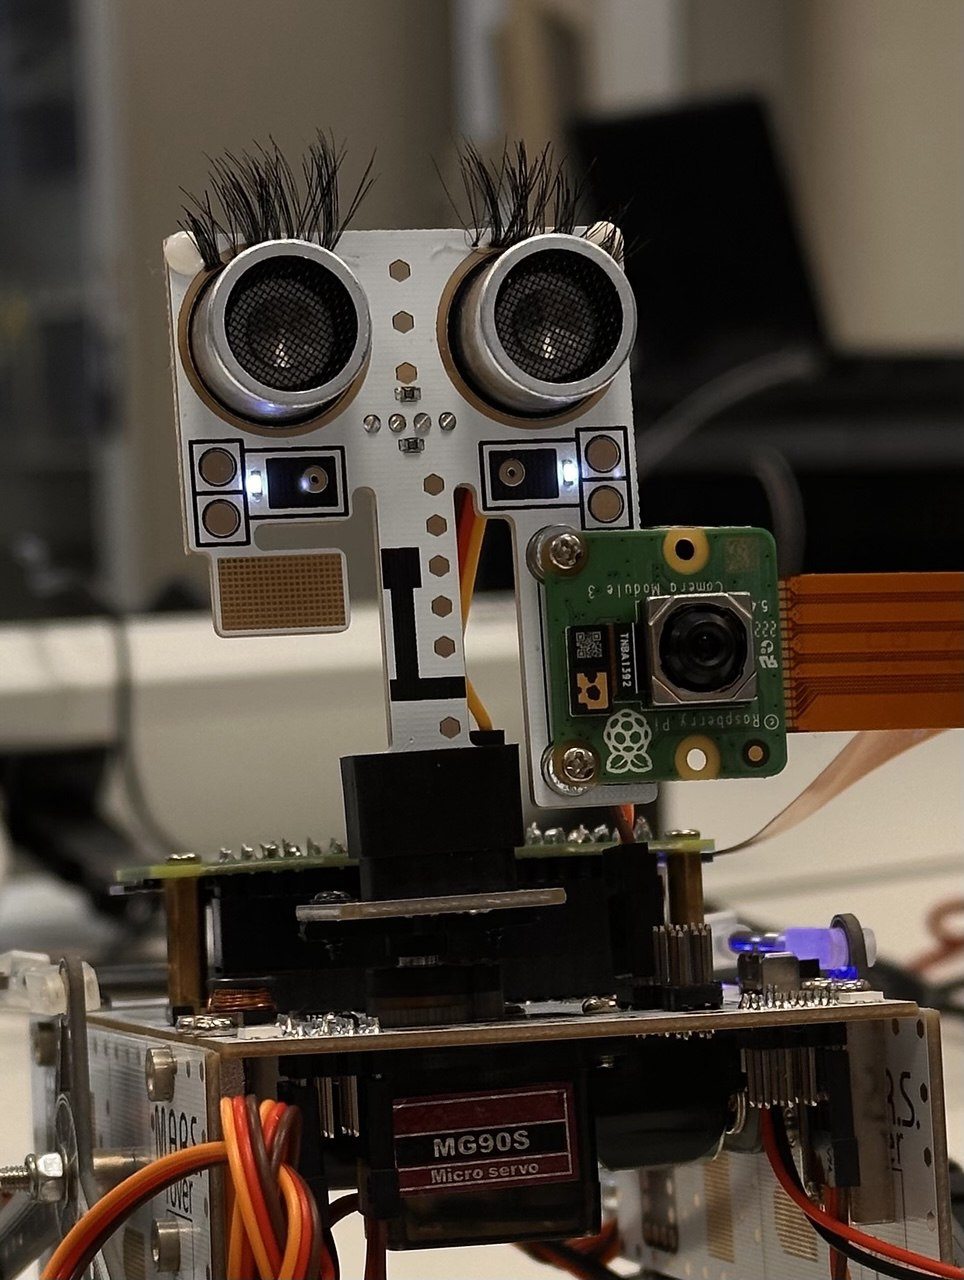
\includegraphics[width=0.4\linewidth]{Hauptkapitel/Pictures/Camera_modul.jpg}
     \caption{Installed Camera Module}
     \label{fig:cam_rover}
 \end{figure}
 
\section{DHT 22 Sensor}

\paragraph{} DHT 22 Sensor has two constructional holes that could be used to attach it to the rover. However, due to the limitations of the rover body, there were only four points of attachment: 4 holes in the corners which originally were made for the keypad. Two in the front were not the best decision, as it would limit the mast's mobility, so the sensor was installed in the back.

